\documentclass[12pt]{article}
\usepackage{hyperref}
\usepackage{graphicx}
\usepackage{parskip}
\usepackage{float}

\hypersetup{
    colorlinks,
    citecolor=black,
    filecolor=black,
    linkcolor=black,
    urlcolor=black
}

\title{PEU 356 Assignment 1}
\author{Mohamed Hussien El-Deeb (201900052)}
\date{\today}

\begin{document}

\maketitle
\tableofcontents

\section{3.10.1}

\subsection{a}

\(u\) curves are \(\frac{n}{x}\) asymptotes, \(u=0\) is xz-plane, repeated for all values of \(z\).

\[
    (x, \frac{u_i}{x}, z)
\]

\(v\) curves are x shaped for \(v=0\), horizontal hyperbola for \(v>0\), vertical hyperbola for \(v<0\), repeated for all values of \(z\).

\[
    (x, \pm\sqrt{x^2 - v_i}, z)
\]

\(z\) curves are planes parallel to xy-plane.


\[
    (x, y, z_i)
\]

\subsection{b}

\begin{figure}[H]
    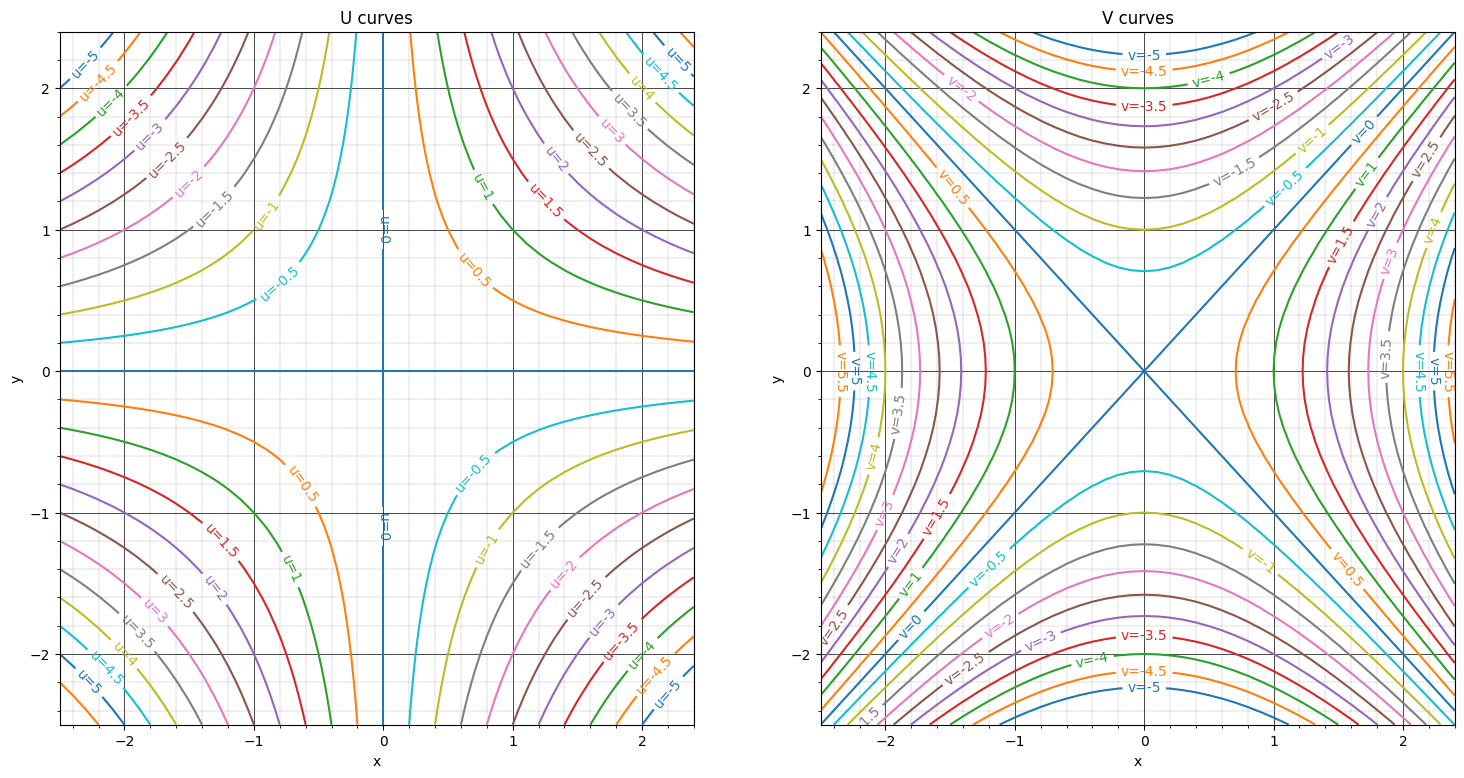
\includegraphics[width=\linewidth]{Q1B.png}
    \caption{U and V curves.}
    \label{fig:Q1B}
\end{figure}

\begin{figure}[H]
    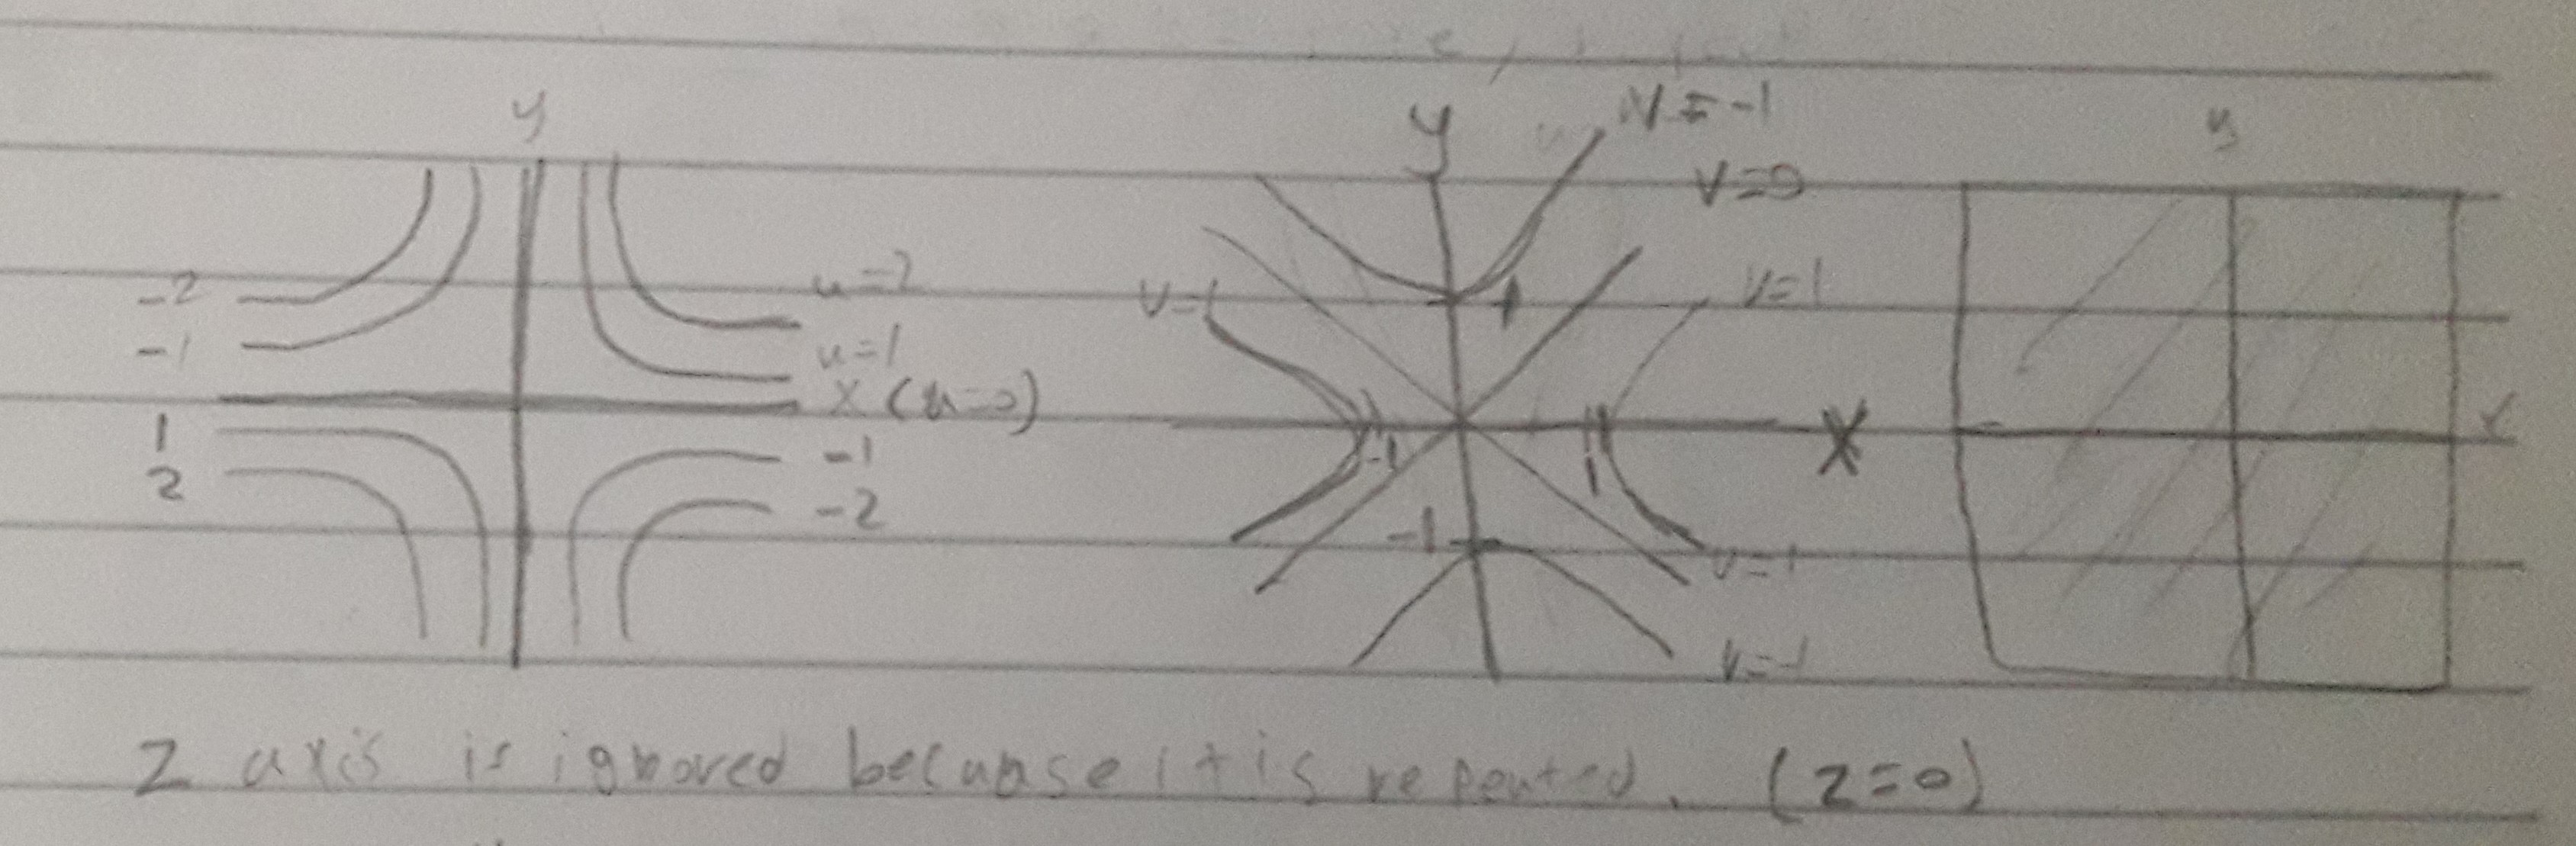
\includegraphics[width=\linewidth]{Q1B.jpg}
    \caption{U and V curves sketch.}
    \label{fig:Q1B2}
\end{figure}

\subsection{c}

\subsection{d}

\section{3.10.4}

\subsection{a}

\subsection{b}

\section{3.10.5}

\section{3.10.28}

\section{3.10.29}

\section{3.10.30}

\subsection{a}

\subsection{b}

\section{3.10.31}

\section{3.10.32}

\subsection{a}

\subsection{b}

\subsection{c}

\end{document}